\documentclass[english]{beamer}
\usetheme{Madrid}

\usepackage{amsmath}
\usepackage{amsfonts}
\usepackage{amssymb}
\usepackage{amsthm}
\usepackage{subcaption}
\usepackage{svg}
\usepackage{csquotes}
\usepackage{babel}
\usepackage[noabbrev, capitalise]{cleveref}

\usepackage[style = numeric,
citestyle=numeric,
sorting=nyt,
sortcites=true,
autopunct=true,
hyperref=true,
abbreviate=false,
backend=biber,
isbn=false,
url=false,
eprint = false,
maxbibnames=99
]{biblatex}
\renewbibmacro{in:}{}
\DeclareSourcemap{
	\maps[datatype=bibtex]{
		\map{
			\step[fieldset=extra, null]
			\step[fieldset=urldate, null]
			\step[fieldset=location, null]
		}
	}
}
\AtEveryBibitem{%
	\clearfield{day}%
	\clearfield{month}%
	\clearfield{endday}%
	\clearfield{endmonth}%
}

\addbibresource{book-embeddings.bib}

\makeatletter
\setbeameroption{show notes on second screen}
\setbeamertemplate{navigation symbols}{}
\setbeamertemplate{page number in head/foot}{}
\setbeamertemplate{title in head/foot}{}
\setbeamertemplate{author in head/foot}{}
\setbeamertemplate{footline}
{%
  \leavevmode%
  \hbox{%
  \begin{beamercolorbox}[wd=1\paperwidth,ht=2.25ex,dp=1ex,center]{author in head/foot}%
  \end{beamercolorbox}%
}%
  \vskip0pt%
}
\makeatother

\newtheorem{conjecture}{Conjecture}

\author{Eric Luu
\\[1 cm]
\footnotesize{Supervisor: Prof. David Wood}
}
\title{Structural Graph Theory and Book Embeddings}

\begin{document}

\frame{\titlepage}

\begin{frame}
  \frametitle{Graphs}

  \begin{columns}
    \begin{column}{0.5\textwidth}
      \begin{itemize}
        \item Graph $G = (V(G), E(G))$
        \item Planar graph: Graph embedded on plane
        \item Planar graphs are 4-colourable \cite{appelEveryPlanarMap1989}
      \end{itemize}
    \end{column}

    \begin{column}{0.5 \textwidth}
      \begin{figure}
        \centering
        \includesvg[width = 0.8\linewidth]{figures/facetriangulation.svg}
      \end{figure}
    \end{column}
  \end{columns}
\end{frame}

\begin{frame}
  \frametitle{Minors}
  \begin{columns}
    \begin{column}{0.5\textwidth}
      \begin{itemize}
        \item $H$ is a \textbf{minor} of $G$ if $H$ is obtained from $G$ through:
              \begin{itemize}
                \item vertex deletion
                \item edge deletion
                \item edge contraction
              \end{itemize}
              \begin{figure}
                \centering
                \includesvg[width = 0.7\textwidth]{figures/edge_contraction.svg}
              \end{figure}
      \end{itemize}
    \end{column}
    \pause
    \begin{column}{0.5\textwidth}
      \begin{itemize}
        \item Minor-closed class = closed under minor relation
        \item Examples of Minor-closed classes:
              \begin{itemize}
                \item Planar graphs
                \item Linkless graphs
                \item Knotless graphs
              \end{itemize}
        \item \textcite{kuratowskiProblemeCourbesGauches1930,wagnerUeberEigenschaftEbenen1937}: $G$ planar iff $G$ $\{K_5, K_{3,3}\}$-minor-free
      \end{itemize}
    \end{column}
  \end{columns}
  \note{mention minimal forbidden minors + graph minor theorem}
\end{frame}

\begin{frame}
  \frametitle{Surfaces}
  \begin{columns}
    \begin{column}{0.5\textwidth}
      \begin{itemize}
        \item Surface = 2D manifold
        \item Examples: \begin{itemize}
                \item Sphere
                \item Torus
                \item Projective Plane
              \end{itemize}
              \begin{figure}
                \centering
                \includesvg[width = 0.8\linewidth]{figures/surfaces.svg}
                \caption{Surfaces}
              \end{figure}
      \end{itemize}
    \end{column}
    \pause
    \begin{column}{0.5 \textwidth}
      \begin{itemize}
        \item Extend planar graphs to any surface
        \item Embed graph on surface
        \item Graphs on surface = Minor-closed class
      \end{itemize}
      \begin{figure}
        \centering
        \includesvg[width = 0.8\linewidth]{figures/k6_projective_plane.svg}
        \caption{$K_6$ embedded on graph}
      \end{figure}
    \end{column}
  \end{columns}
  \note{35 forbidden minors for projective plane, $\geq 16 \, 000$ torus}
\end{frame}

\begin{frame}
  \frametitle{Books}
  \begin{columns}
    \begin{column}{0.5\textwidth}
      \begin{itemize}
        \item Book: half-planes glued on boundary
        \item Half Planes: Pages
        \item Book-embedding: Graph on book
        \item Smallest no. pages to embed $G$ = pagenumber $G$
      \end{itemize}
    \end{column}
    \pause
    \begin{column}{0.5\textwidth}
      \begin{figure}
        \centering
        \includesvg[height = 0.7\textheight]{figures/3page_K5.svg}
        \caption{From \textcite{eppsteinBookEmbedding2014}}
      \end{figure}
    \end{column}
  \end{columns}
  \note{Books were introduced by Persinger + Atneosen in the 1960s
    Book-embeddings were introduced by Kainen and Ollman in the 1970s.
  }
\end{frame}


\begin{frame}
  \frametitle{Planar Book-Embeddings}
  \begin{columns}
    \begin{column}{0.5\textwidth}
      \begin{itemize}
        \item Planar Graphs can be embedded on four pages \cite{yannakakisEmbeddingPlanarGraphs1989}
        \item Bound is tight! \cite{yannakakisPlanarGraphsThat2020,bekosFourPagesAre2020}
      \end{itemize}

      \begin{figure}
        \centering
        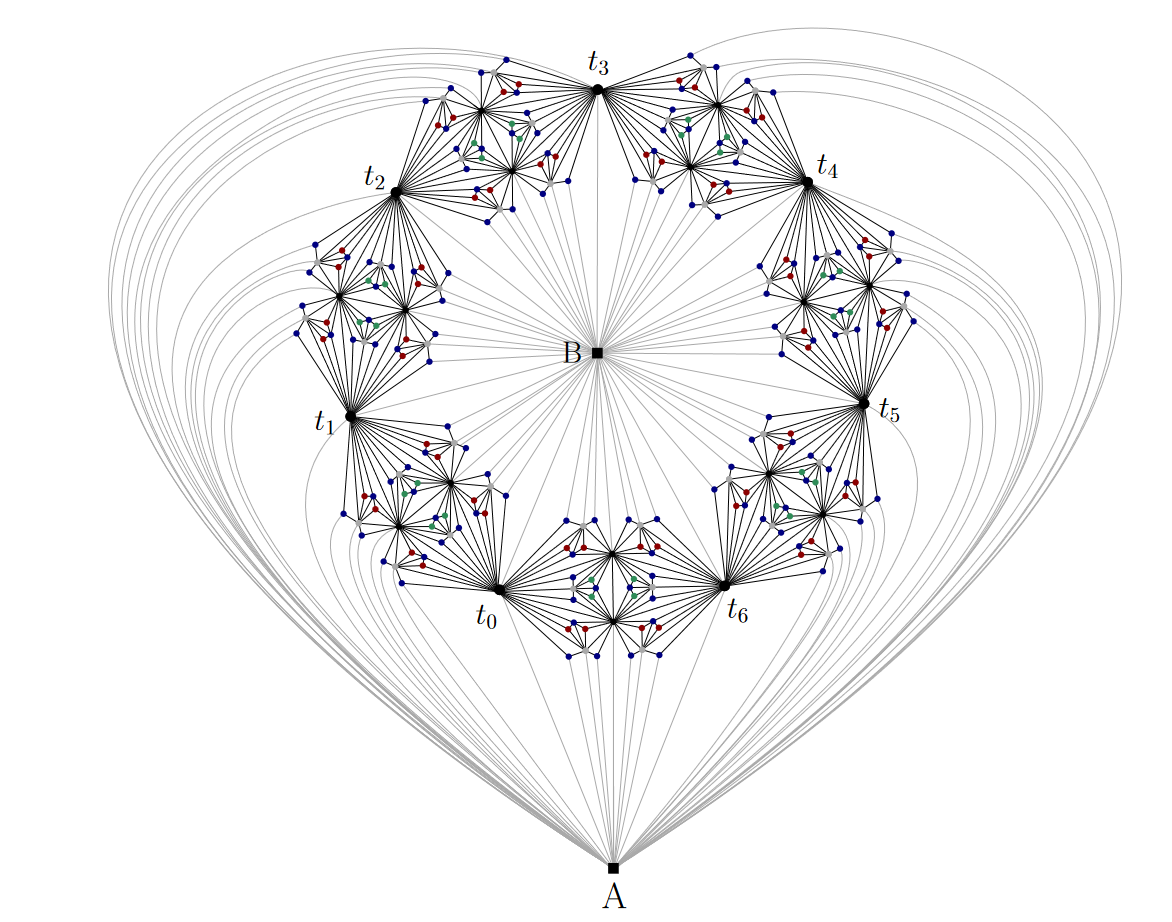
\includegraphics[width = \linewidth]{figures/Screenshot 2024-09-26 152422.png}
        \caption{Planar graph with pagenumber 4, from \cite{bekosFourPagesAre2020}}
      \end{figure}
    \end{column}
    \pause
    \begin{column}{0.5\textwidth}
      \begin{itemize}
        \item Graphs embedded on surface with orientable genus $g$ can be embedded on $O(g)$ pages \cite{heathPagenumberGenusGraphs1992}
        \item Projective-planar graphs can be embedded on 6 pages \cite{ozekiBookEmbeddingGraphs2019}
      \end{itemize}
    \end{column}
  \end{columns}
  \note{
    Proven by Yannakakis in 2020, other paper with authors Bekos, Kaufmann, Klute, Pupyrev, Raftopoulou, Uedkerdt also proved this in 2020.
    Mention Nakamoto, Nozawa
  }
\end{frame}

\begin{frame}
  \frametitle{Main Conjecture}
  \begin{conjecture}
    If $G$ is in minor-closed class $\mathcal{G}$, then $G$ is embeddable on $f(\mathcal{G})$ pages.
  \end{conjecture}
  \note{Minor-closed family is family closed under taking minors
    Examples of minor-closed families: planar graphs, Graphs embedded on surfaces etc.}
\end{frame}

\begin{frame}
  \frametitle{Graph Minor Structure Theorem}
  \begin{columns}
    \begin{column}{0.5\textwidth}
      \begin{itemize}
        \item Minor-closed class $\implies$ $K_t$-minor-free
        \item $K_t$-minor-free graphs can be built from 4 ingredients \cite{robertsonGraphMinorsXVII1999} \begin{itemize}
                \item Graphs on surfaces
                \item Vortices on surfaces
                \item Apex sets
                \item Clique-Sums
              \end{itemize}
      \end{itemize}
    \end{column}
    \begin{column}{0.5\textwidth}
      \begin{figure}
        \centering
        \includesvg[width = 0.8\textwidth]{figures/Clique-sum.svg}
        \caption{Clique sums, \cite{eppsteinCliquesum2023}}
      \end{figure}
    \end{column}
  \end{columns}
  \note{mention rough characterisation, numbers get very big}
\end{frame}

\begin{frame}
  \begin{conjecture}
    Every graph embedded on $\Sigma$ can be embedded on $k(\Sigma)$ pages with every face having a bounded number of pairwise nesting edges.
  \end{conjecture}
\end{frame}

\begin{frame}[shrink = 50]

  \printbibliography
\end{frame}

\end{document}